%!TEX program = xelatex
% 完整编译: xelatex -> bibtex -> xelatex -> xelatex
\documentclass[lang=cn,11pt,a4paper,cite=numbers]{elegantpaper}
\title{ZJU课程论文模板}
% 作者与单位
\author{xxx  xxxxxxxx}
\institute{浙江大学软件学院}

% 版本号
% \version{0.9}
\version{}
% 日期
% \date{\zhtoday}
\date{}

% 本文档命令
\usepackage{array}
\newcommand{\ccr}[1]{\makecell{{\color{#1}\rule{1cm}{1cm}}}}





\begin{document}

\maketitle

\begin{abstract}摘要摘要摘要摘要摘要摘要摘要摘要摘要摘要摘要摘要摘要摘要摘要摘要摘要摘要摘要摘要摘要摘要摘要摘要摘要摘要摘要摘要摘要摘要摘要摘要摘要摘要摘要摘要摘要摘要摘要摘要摘要摘要摘要摘要摘要摘要摘要摘要摘要摘要摘要摘要摘要摘要摘要摘要摘要摘要摘要摘要摘要摘要摘要摘要摘要摘要摘要摘要摘要摘要摘要摘要摘要摘要摘要摘要摘要摘要摘要摘要摘要摘要摘要摘要摘要摘要摘要摘要摘要摘要摘要摘要摘要摘要摘要摘要摘要摘要摘要摘要摘要摘要摘要摘要摘要摘要摘要摘要摘要摘要摘要摘要摘要摘要摘要摘要摘要摘要摘要摘要摘要。
\keywords{latex,工作论文,模板}
\end{abstract}

\section{第一章}
第一章第一章第一章第一章第一章
\subsection{第一章第一节}
第一章第一节第一章第一节第一章第一节第一章第一节
\subsubsection{小小节}
这里是第一段这里是第一段这里是第一段这里是第一段

\subsection{第一章第二节}
第一章第二节第一章第二节第一章第二节第一章第二节 \footnote{可以使用命令提示符,输入调出本地宏包文档}

这里有一个脚注。
\subsubsection{小小节}
\paragraph{}这里是第一段这里是第一段这里是第一段这里是第一段


\section{这里演示代码}
这里是第一段。
\begin{lstlisting}
 // @lc code=start
 class Solution {
     // 一种高效的解法
     public boolean isPalindrome(int x) {
         if (x < 0 || (x % 10 == 0 && x != 0)) return false;
         int rev = 0;
         while (x > rev) {
             rev = rev * 10 +  x % 10;
             x /= 10;
         }
         return x == rev || x == rev / 10;
     } 
 }
 // @lc code=end
 
 
\end{lstlisting}


\section{这里演示标号}
\subsection{第一种}
\begin{enumerate}[label=\arabic*).]
  \item \textit{如何删除版本信息?}\\
    xxxxxxxxxxxx
  \item \textit{如何删除日期?}\\
    xxxxxxxxxxxx
  \item \textit{如何获得中文日期?}\\
    xxxxxxxxxxxx
\end{enumerate}
\subsection{第二种}
\begin{enumerate}
  \item math=cm
  \item math=newtx
  \item math=mtpro2
\end{enumerate}

\section{这里演示图片}
这里演示图片这里演示图片这里演示图片这里演示图片这里演示图片这里演示图片这里演示图片这里演示图片这里演示图片这里演示图片这里演示图片这里演示图片这里演示图片这里演示图片这里演示图片这里演示图片这里演示图片这里演示图片这里演示图片这里演示图片这里演示图片这里演示图片。
\begin{figure}[!htb]
\centering
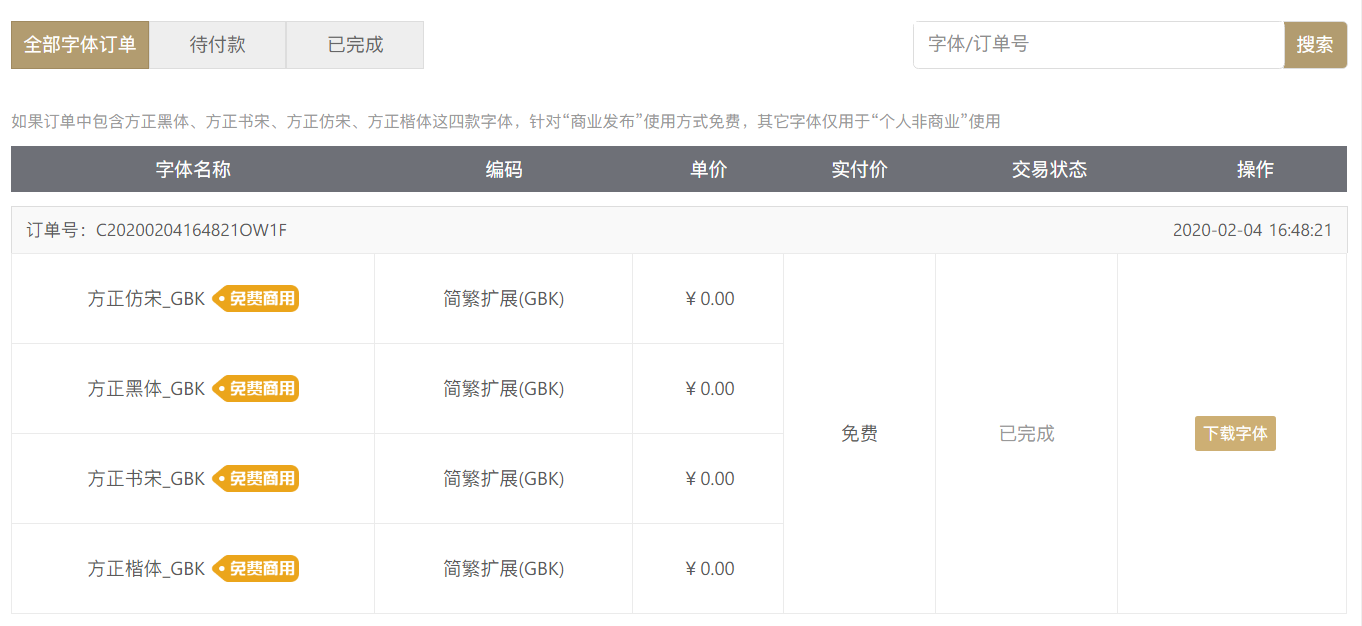
\includegraphics[width=0.9\textwidth]{founder.png}
\caption{这里是图1}
\end{figure}


\section{这里演示表格}
这里演示表格这里演示表格这里演示表格这里演示表格这里演示表格这里演示表格这里演示表格这里演示表格这里演示表格这里演示表格这里演示表格这里演示表格这里演示表格这里演示表格这里演示表格这里演示表格这里演示表格3。

\begin{table}[!htb]
  \centering
  \caption{Elegant\LaTeX{} 表格模板}
    \begin{tabular}{*{4}{>{\scriptsize}c}}
    \hline
    \textbf{姓名} & \textbf{年龄} & \textbf{日期} & \textbf{QQ}\\
    \hline
    Sam  & 10 & 2019/05/15 & 123456  \\
    Tim    & 20 & 2019/05/27 & 123456 \\
    Sam  & 10 & 2019/05/15 & 123456  \\
    Tim    & 20 & 2019/05/27 & 123456 \\
    Sam  & 10 & 2019/05/15 & 123456  \\
    Tim    & 20 & 2019/05/27 & 123456 \\
    Sam  & 10 & 2019/05/15 & 123456  \\
    Tim    & 20 & 2019/05/27 & 123456 \\
    \hline
    \end{tabular}%
  \label{tab:donation}%
\end{table}%

\section{引用参考文献}
引用参考文献1\cite{ref1}

引用参考文献2\cite{ref1, ref4}


\begin{thebibliography}{99}  
  \bibitem{ref1}Zheng L, Wang S, Tian L, et al., Query-adaptive late fusion for image search and person re-identification, Proceedings of the IEEE Conference on Computer Vision and Pattern Recognition, 2015: 1741-1750.  
  \bibitem{ref2}Arandjelović R, Zisserman A, Three things everyone should know to improve object retrieval, Computer Vision and Pattern Recognition (CVPR), 2012 IEEE Conference on, IEEE, 2012: 2911-2918.  
  \bibitem{ref3}Lowe D G. Distinctive image features from scale-invariant keypoints, International journal of computer vision, 2004, 60(2): 91-110.  
  \bibitem{ref4}Philbin J, Chum O, Isard M, et al. Lost in quantization: Improving particular object retrieval in large scale image databases, Computer Vision and Pattern Recognition, 2008. CVPR 2008, IEEE Conference on, IEEE, 2008: 1-8.  
  \end{thebibliography}

\end{document}
